% KDMiLe submission -- condensed version of the author's undergraduate thesis (TCC)
% Structure based on template-kdmile.tex (kdmile.cls)

\documentclass[kdmile,a4paper]{kdmile} % NOTE: kdmile is published on A4 paper
\usepackage{graphicx,url}
\usepackage[T1]{fontenc}
\usepackage{amsmath,amssymb}
\usepackage{booktabs,flafter}
% O template fixa rodapé e aviso editorial de 2025; esta é uma versão de trabalho.
\makeatletter
\def\runningfoot{\def\@runningfoot{Manuscrito revisado, outubro de 2026.}}
\def\firstfoot{\def\@firstfoot{Manuscrito revisado, outubro de 2026.}}
\long\def\permission{\par Versão de trabalho para revisão dos autores.}
\makeatother

% ====================================================================
% Author metadata (3 authors: student + advisor + co-advisor, all UTFPR,
% same institution -- so \inst{} indices are omitted, per the template's
% "both authors belong to the same university" convention, Section 2).
% Abbreviation follows the KDMiLe rule for 2-3 authors (each given name
% reduced to its initial, full surname kept exactly as spelled in the
% TCC's variaveis.tex: "João Victor Dos Santos Gomes", "Jorge Aikes
% Junior", "Davi Pereira dos Santos").
% NOTE: confirm with your advisors whether they wish to be listed as
% co-authors of the article (common for TCC-derived papers) or only
% acknowledged; adjust \author/\institute/\ack accordingly if needed.
% ====================================================================

\markboth{J. V. Dos Santos Gomes and J. Aikes Junior and D. Pereira dos Santos}
{Ranking Classification Pipelines with Statistical Dataset Embeddings: A Meta-Learning Approach}

\title{Ranking Classification Pipelines with Statistical Dataset Embeddings:\\ A Meta-Learning Approach}

\author{J. V. Dos Santos Gomes, J. Aikes Junior, D. Pereira dos Santos}

\institute{Universidade Tecnológica Federal do Paraná (UTFPR), Brazil \\
\email{joaogomes.2003@alunos.utfpr.edu.br, jorgejunior@utfpr.edu.br, davip@professores.utfpr.edu.br}
}

% Article abstract (100-300 words, English, no references, single paragraph)
\begin{abstract}
Selecting classification pipelines requires evaluating both data representation and predictor choice. We revisit a statistical meta-learning benchmark containing 201 OpenML tasks and 60 pipelines. Dataset vectors comprise 55 deterministic descriptors and nine padded zeros, with no representation learning. Auditing related tasks and minimum class support yields a primary evaluation of 193 tasks in 165 groups. Five outer group partitions, with inner group validation for neighborhood selection, compare multi-output k-NN and Random Forest against global-mean and random baselines. Group-averaged weighted Kendall is 0.3995 for k-NN, 0.4309 for Random Forest and 0.3690 for the global mean. The paired Random Forest minus k-NN difference is 0.0314 with a descriptive 95\% interval [0.0073, 0.0564]; the k-NN advantage over the global mean remains uncertain. Error analysis identifies 17 tasks with nonpositive weighted correlation and one undefined case. A separate 180-evaluation pilot explores hyperparameters on raw data with preprocessing fitted within folds. Historical Phase 1 scores remain subject to preprocessing and sampling limitations; the results characterize this retrospective benchmark rather than establish universal superiority.
\end{abstract}

% ACM Computing Classification System (CCS) categories
\begin{CCSXML}
	<ccs2012>
	<concept>
	<concept_id>10010147.10010257.10010321</concept_id>
	<concept_desc>Computing methodologies~Machine learning algorithms</concept_desc>
	<concept_significance>500</concept_significance>
	</concept>
	<concept>
	<concept_id>10002951.10003317.10003347.10003352</concept_id>
	<concept_desc>Information systems~Learning to rank</concept_desc>
	<concept_significance>300</concept_significance>
	</concept>
	</ccs2012>
\end{CCSXML}

\ccsdesc[500]{Computing methodologies~Machine learning algorithms}
\ccsdesc[300]{Information systems~Learning to rank}

% Keywords (alphabetical order)
\keywords{AutoML, dataset embeddings, k-nearest neighbors, meta-learning, pipeline ranking}

\begin{document}

\begin{bottomstuff}
% Optional: add a funding/scholarship statement here if applicable
% (e.g., "J. V. dos Santos Gomes was supported by a scholarship from
% PLACEHOLDER_FUNDING_AGENCY, grant nº PLACEHOLDER_NUMBER").
% Leave empty if there is no grant/scholarship to disclose.
\end{bottomstuff}

\maketitle

\section{Introdução}
\label{sec:introduction}

A recomendação de pipelines de classificação combina decisões sobre pré-processamento, seleção de atributos e classificador. Em AutoML, essa escolha depende do espaço de busca, da estratégia e do protocolo de avaliação \cite{Baratchi2024}. O meta-aprendizado reutiliza experiências entre problemas, mas a validade das recomendações depende de separar tarefas relacionadas e de ajustar hiperparâmetros sem consultar o teste.

Este trabalho investiga uma representação estatística determinística para ranquear 60 pipelines e compara preditores k-NN e Random Forest multi-saída. A partir de um acervo histórico de 201 tarefas OpenML, a auditoria delimita 193 tarefas elegíveis em 165 grupos. Spearman e Kendall avaliam a ordenação global, Kendall ponderado enfatiza pares de maior importância e NDCG@5 e regret avaliam utilidade das primeiras recomendações. As métricas são complementares, e NDCG alto não implica recuperar exatamente os melhores pipelines.

As contribuições são: (i) explicitar a construção dos 64 componentes do vetor e os critérios de elegibilidade; (ii) disponibilizar avaliação por grupos com ajuste interno e baselines calculadas no treino; e (iii) documentar erros, resultados ausentes e um piloto de hiperparâmetros. O estudo distingue reprodução histórica de nova avaliação, sem apresentar um caso isolado como validação externa.

\section{Trabalhos Relacionados}

A discussão está organizada em três eixos: representação, recomendação e avaliação. No primeiro, Dataset2Vec aprende representações de conjuntos de dados \cite{Jomaa2021}, enquanto o vetor aqui utilizado concatena estatísticas fixas e não recebe treinamento. TabPFN \cite{Hollmann2025} exemplifica reutilização de conhecimento entre problemas tabulares por um modelo fundacional; sua tarefa de predição difere do ranqueamento do arsenal estudado.

No eixo de recomendação, \citeN{Baratchi2024} oferecem um enquadramento para distinguir espaço de busca, estratégia e avaliação. Este trabalho mantém o arsenal fixo na comparação principal para separar a influência do metamodelo. Isso favorece controle experimental, mas restringe conclusões sobre configurações não avaliadas.

No eixo de avaliação, AMLB \cite{Gijsbers2024} enfatiza comparações extensíveis que consideram desempenho, custo e falhas. Aqui, essa perspectiva orienta a disponibilização de exclusões e predições por tarefa. No Free Lunch não garante, sozinho, vantagem de uma recomendação personalizada em dados reais: seus pressupostos e a relação com vieses indutivos exigem análise cuidadosa \cite{Goldblum2024}. Não se comparam diretamente correlações obtidas em tarefas e protocolos distintos.

\section{Metodologia}

O estudo compreende reprodução do acervo, auditoria, avaliação por grupos e um piloto separado. Configuração, metadados OpenML, índices de divisão, predições e escores ficam em arquivos próprios, ligados por identificadores de tarefa, pipeline, fold e modelo.

\subsection{Acervo Histórico e Critérios de Qualidade}

O acervo tem 201 tarefas do OpenML \cite{Vanschoren2014}, representações $X\in\mathbb{R}^{201\times64}$ e desempenhos $Y\in\mathbb{R}^{201\times60}$. Das 12.060 células, 172 estão ausentes. O carregador histórico codificou categorias e imputou a mediana antes da CV. A SVM recebeu uma subamostra global de até 5.000 exemplos, enquanto outros classificadores usaram o conjunto inteiro. Essas decisões limitam os escores reutilizados; a Fase 1 completa não foi reconstruída.

Os 60 pipelines cruzam quatro escalonadores (StandardScaler, MinMaxScaler, RobustScaler e ausência), três seletores (PCA, SelectKBest por ANOVA e ausência) e cinco classificadores: Random Forest com 100 árvores, SVM RBF com $C=1$ e gamma scale, k-NN com cinco vizinhos, MLP com camadas 64 e 32 e até 200 iterações, e árvore com profundidade máxima 10. PCA e SelectKBest usam $\min(10,\max(1,P-1))$ componentes ou atributos. Os algoritmos estocásticos usam semente 42. Não se realiza otimização dos hiperparâmetros desse arsenal no experimento principal.

Metadados oficiais confirmam classificação supervisionada para as 201 tarefas. Nomes repetidos ou fingerprints idênticos dos atributos processados formam grupos transitivos conservadores. São 186 nomes e 172 grupos no acervo. A avaliação principal requer 500--10.000 exemplos, ao menos duas classes e mínimo de cinco exemplos por classe. Excluem-se oito tarefas (2075, 3486, 362281, 363078, 363094, 363393, 363554 e 363559), sem consultar seu desempenho de ranking. Restam 193 tarefas, 179 nomes, 165 grupos e 52 escores ausentes. O catálogo inclui links de tarefa e conjunto, tamanho, dimensionalidade, classes, balanceamento e motivos de exclusão.

A tarefa 363713 já consta no acervo e não constitui holdout independente. Sua demonstração pontual foi removida. O agrupamento reduz repetições detectáveis, mas não certifica independência entre todas as possíveis versões dos conjuntos.

\subsection{Representação Estatística de 64 Posições}

Para cada atributo numérico, calculam-se nove descritores: média, desvio padrão populacional acrescido de $10^{-8}$, mínimo, máximo, mediana, assimetria, curtose de Fisher e correlações de Pearson e Spearman com o alvo codificado. Cada descritor é agregado entre atributos por mínimo, percentil 25, média, percentil 75 e máximo, produzindo 45 entradas.

Dez propriedades globais completam o vetor: $\log(1+N)$, $\log(1+P)$, número de classes, proporções majoritária e minoritária, entropia das proporções acrescidas de $10^{-8}$, proporção de atributos constantes, média da matriz de correlação absoluta entre atributos com diagonal zerada, média das proporções de valores únicos e $P/(N+10^{-8})$. A média das correlações inclui os zeros da diagonal no denominador $P^2$.

Concatenam-se 55 descritores e nove zeros; com dimensão 64 não há truncamento. Aplica-se \texttt{nan\_to\_num} e normalização L2, preservando vetor nulo. Os percentis por atributo calculados no código não integram os nove blocos. Não há loss, pesos aprendidos ou treinamento da representação. O método exige rótulos do conjunto consultado, e correlações com códigos nominais multiclasses dependem de uma ordenação arbitrária.

\subsection{Preditores e Validação por Grupos}

O k-NN prevê a acurácia de cada pipeline pela média dos vizinhos ponderada por $w_i=1/(d_i+10^{-8})$, com distância euclidiana. O comparador Random Forest é um regressor multi-saída nativo com 200 árvores, mínimo de duas observações por folha, \texttt{max\_features=1.0} e semente 42. A média global usa somente o treino; o baseline aleatório usa escores uniformes com semente 42 acrescida do fold.

Usa-se GroupKFold externo com cinco divisões, embaralhamento e semente 42. Dentro de cada treino externo, quatro divisões por grupos escolhem $k\in\{1,3,5,7,10\}$ pela média de Kendall ponderado por grupo; empates escolhem o menor $k$. Avalia-se também um k-NN cujas dimensões são padronizadas exclusivamente no treino de cada divisão. Nenhum grupo de teste é usado para ajustar k, imputação ou padronização.

Escores ausentes de treino são imputados pela mediana por pipeline. Colunas inteiramente ausentes no treino ficam fora da avaliação do teste. Escores reais ausentes não são imputados para calcular métricas. Correlações indefinidas são mantidas como NaN com estado explícito, preservando NDCG e regret quando calculáveis. As médias são agregadas primeiro dentro de grupo, depois entre grupos.

\subsection{Métricas e Análise de Erros}

Spearman mede associação de postos e Kendall tau-b trata empates. O Kendall ponderado padrão da SciPy usa pesos hiperbólicos aditivos $1/(r_i+1)+1/(r_j+1)$ e média de duas ordenações lexicográficas decrescentes dos escores real e predito; não usa produto dos postos e não fornece p-valor.

NDCG é calculado pela implementação do scikit-learn com ganho linear da acurácia balanceada:
\begin{equation}
\operatorname{DCG}@K=\sum_{i=1}^{K}\frac{rel_i}{\log_2(i+1)},\qquad
\operatorname{NDCG}@K=\frac{\operatorname{DCG}@K}{\operatorname{IDCG}@K}.
\end{equation}
Reportam-se NDCG completo, NDCG@5 e regret: melhor acurácia real disponível menos a acurácia da primeira recomendação (ou da melhor entre cinco). Empates de predição recebem tratamento médio em NDCG e ordem estável das colunas em regret. Assim, NDCG e Kendall ponderado capturam aspectos complementares da ordenação.

Intervalos descritivos de 95\% usam 2.000 reamostragens de grupos com semente 42; diferenças pareadas usam grupos com ambas as métricas definidas. A sobreposição de treinos limita a inferência. O diagnóstico considera tamanho, número de atributos, proporção majoritária, atributos constantes e distância ao vizinho. Correlações exploratórias por grupo recebem ajuste Benjamini--Hochberg para cinco comparações, sem interpretação causal.

\section{Resultados e Discussão}

Esta seção apresenta a reprodução histórica, a comparação principal e o diagnóstico de falhas. O piloto de hiperparâmetros é discutido separadamente, pois utiliza dados brutos e não substitui os escores do acervo.

\subsection{Reprodução e Comparação Principal}

A reprodução com o preditor KDTree original mantém, para $k=10$, Spearman médio de aproximadamente 0,5801 e Kendall ponderado de 0,5222 sobre 198 tarefas com correlações definidas. Esses resultados por tarefa podem manter parentes no treino e escolher k na mesma avaliação; são exploração histórica. Diferenças para a nova avaliação também refletem o tamanho de treino, os filtros e a agregação, não apenas o agrupamento.

A Tabela~\ref{tab:modelos} compara os modelos na avaliação revisada. Há 192 tarefas em 164 grupos com correlações definidas, além de um caso de escores reais constantes. NDCG e regret continuam registrados nesse caso. O ajuste interno escolheu $k=10$ nos cinco folds, coincidindo com o k-NN fixo em 10.

\begin{table}[htbp]
\caption{Avaliação revisada: médias por grupo. Menor regret é melhor.}
\label{tab:modelos}
\centering
\resizebox{\linewidth}{!}{\begin{tabular}{lrrrr}
\toprule
Método & Spearman & $\tau_w$ & NDCG@5 & Regret@1 \\
\midrule
Aleatório & $-0.0129$ & $0.0024$ & $0.8687$ & $0.0849$ \\
Média global & $0.4000$ & $0.3690$ & $0.9396$ & $0.0334$ \\
k-NN ajustado & $0.4637$ & $0.3995$ & $0.9355$ & $0.0372$ \\
k-NN padronizado & $0.4736$ & $0.4138$ & $0.9343$ & $0.0339$ \\
Random Forest & $0.4822$ & $0.4309$ & $0.9414$ & $0.0305$ \\
\bottomrule
\end{tabular}}
\end{table}

A diferença pareada Random Forest menos k-NN em Kendall ponderado é 0,0314, com intervalo descritivo [0,0073; 0,0564]. A diferença média global menos k-NN é -0,0305, com intervalo [-0,0637; 0,0026], sem estabelecer vantagem do k-NN nesse critério. A Figura~\ref{fig:modelos} apresenta os intervalos por grupo. O resultado sugere vantagem do Random Forest neste acervo; não demonstra superioridade universal nem isola o efeito da representação, mantida igual em todos os modelos.

\begin{figure}[htbp]
\centering
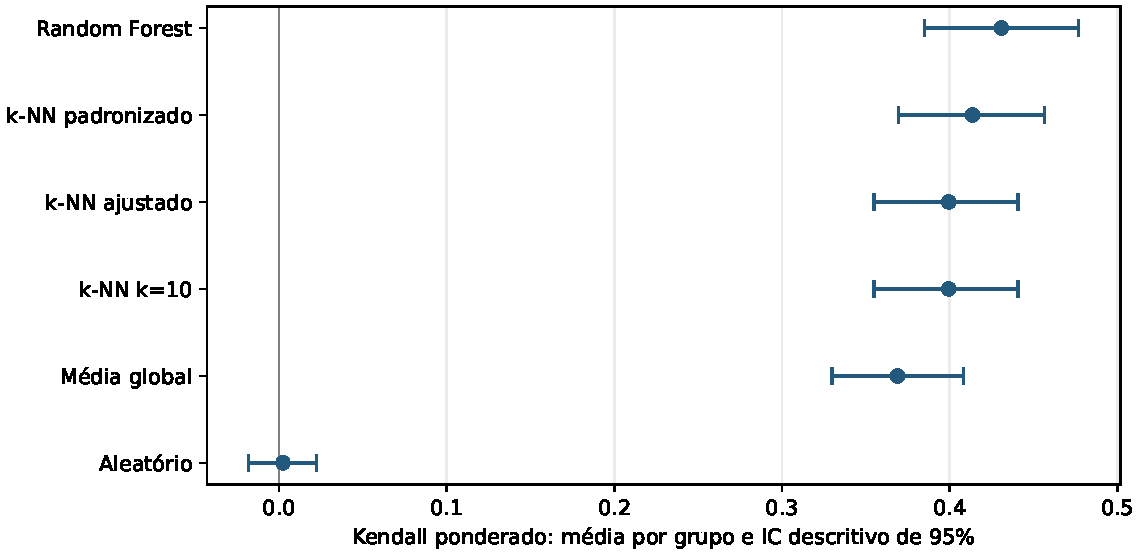
\includegraphics[width=.95\linewidth]{../projeto/resultados/revisao_2026/figuras/comparacao_modelos.pdf}
\caption{Kendall ponderado médio por grupo e intervalos descritivos de 95\%.}
\label{fig:modelos}
\end{figure}

A baseline aleatória já alcança NDCG@5 de 0,8687, o que evidencia a baixa discriminação de NDCG com relevâncias próximas. Portanto, valores altos não demonstram top-5 correto. Regret@1 é 0,0372 para k-NN, 0,0305 para Random Forest e 0,0334 para média global. A interpretação depende conjuntamente de correlação, relevância e perda da recomendação.

\subsection{Diagnóstico e Piloto de Hiperparâmetros}

O k-NN ajustado apresenta 17 tarefas com Kendall ponderado não positivo e uma indefinida. Entre as piores estão as tarefas 363159, 361148 e 361169. Após ajuste das cinco correlações exploratórias, o número de atributos apresenta associação positiva com a qualidade ($\rho\approx0,2064$, $q\approx0,0400$). Não se encontrou associação ajustada abaixo de 0,05 para as demais variáveis. A investigação não permite atribuir falhas exclusivamente a outliers ou desbalanceamento.

No piloto separado, as tarefas 11, 15, 37, 4538, 9914 e 361198 usam dados brutos com o alvo oficial da tarefa. Codificação ordinal categórica e imputação numérica por mediana são ajustadas dentro dos folds. Com StandardScaler e sem seletor, variam-se profundidade da árvore (5, 10, ilimitada) e vizinhos do classificador k-NN (3, 5, 11), totalizando 36 combinações de tarefa/classificador/valor e 180 avaliações nos mesmos cinco folds por tarefa. Os resultados mostram sensibilidade às configurações, mas selecionar o melhor valor nesses folds é exploratório; o piloto não mede ranqueamento de um arsenal expandido em todos os grupos.

\subsection{Limitações}

A representação fixa e o arsenal controlado permitem auditoria e comparação de preditores. Seu alcance é delimitado por rótulos necessários na consulta, codificação nominal arbitrária e pelo espaço de candidatos. A comparação não substitui uma ablação de representações. Os escores históricos mantêm imputação anterior à CV e subamostragem exclusiva da SVM. O piloto corrige o tratamento no subconjunto, mas a matriz completa não foi reconstruída. Os grupos podem não detectar todas as versões relacionadas; a avaliação é retrospectiva, sem teste externo posterior, e Random Forest não foi otimizado. Intervalos por grupo são descritivos devido à sobreposição de treinos.

\section{Conclusão}

O estudo disponibiliza um benchmark auditado para investigação de recomendação de pipelines. Na avaliação revisada, Random Forest apresenta Kendall ponderado médio superior ao k-NN, enquanto a vantagem do k-NN sobre média global permanece incerta pelo intervalo utilizado. A auditoria de grupos, classes raras e demonstração de holdout alterou a interpretação dos resultados e delimitou quais evidências sustentam as conclusões.

Como continuação, propõem-se: (i) reconstruir toda a Fase 1 com pré-processamento dentro dos folds; (ii) ampliar o arsenal de hiperparâmetros; (iii) comparar representações sob o mesmo protocolo; e (iv) testar em conjuntos externos coletados após o desenvolvimento. O acervo histórico, a nova avaliação e o piloto permanecem separados para permitir inspeção e reprodução.

\begin{ack}
Os autores agradecem à Universidade Tecnológica Federal do Paraná pelo apoio institucional e à orientação do TCC que deu origem a este estudo.
\end{ack}
\begin{received}
\end{received}
\bibliographystyle{kdmile}
\bibliography{references}
\end{document}
